\graphicspath{{img}}

\begin{tcolorbox}
Die Produktfunktionen beschreiben jede einzelne Funktion des Produkts mittels Anwendungsfalldiagrammen und Anwendungsfalltabellen.
Diese sollen möglichst ausschlaggebend für das zu entwickelnde System sein und nicht simple Produktfunktionen wie z.B. Login, Account erstellen, Gruppe beitreten, Passwort ändern oder ähnliches zeigen.
\autoref{fig:anwendungsfall-app-tabelle-xx-1} stellt eine exemplarische Tabelle für die Beschreibung eines Anwendungsfalls dar. Stil und Formatierung sind variabel. Nicht jede Zelle muss immer gefüllt sein.
\\\\
In  Tabelle~\autoref{fig:akteur-tabelle} werden alle auftretenden Akteure beschrieben.


\end{tcolorbox}

\begin{figure}[h]
	\centering
	
	\begin{tabularx}{\textwidth}{ p{.2\textwidth} | p{.2\textwidth} | X }
		\textbf{Akteur} & \textbf{Beschreibung} & \textbf{Verwendet in Anwendungsfall} \\ \hline
		Informatiker & Programmiert tolle Sachen & Programmieren, Kaffee trinken, Schlafen
	\end{tabularx}
	
	\caption{Beschreibung der Akteure}
	\label{fig:akteur-tabelle}
\end{figure}

\newpage

\section{Anwendungsfalldiagramm - App}

\begin{figure}[h]
	\centering
    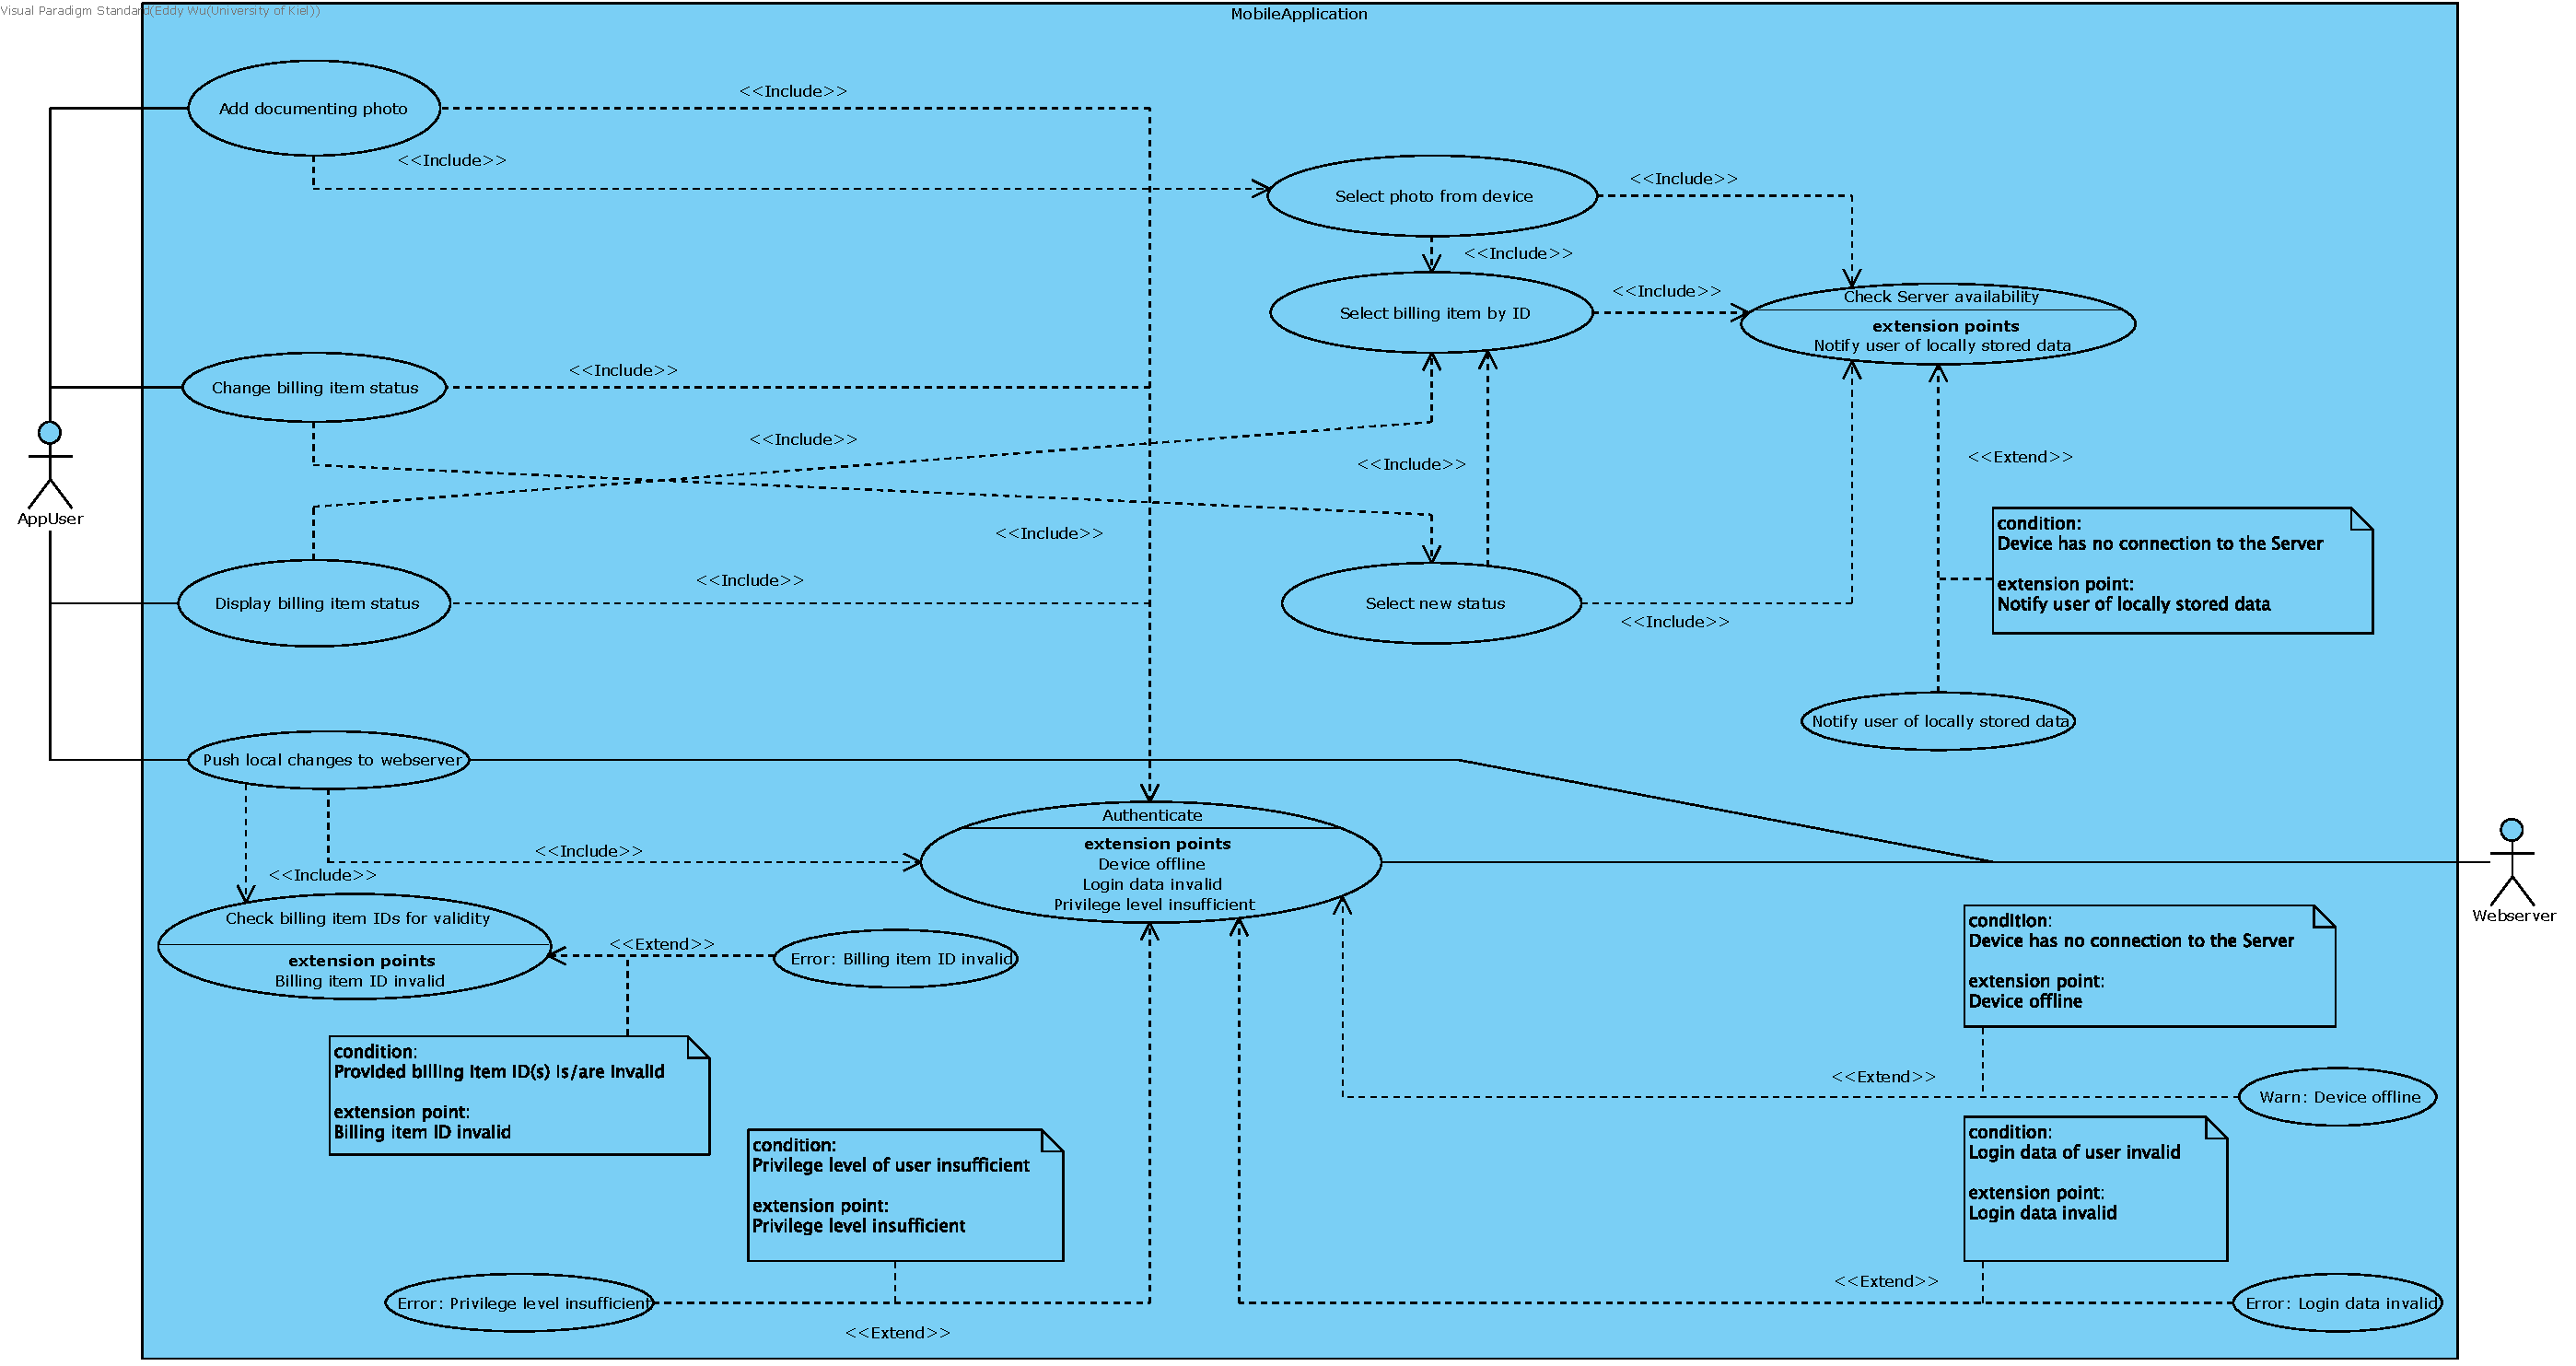
\includegraphics[width=\linewidth]{diagrams/Mobile_Application.pdf}
	\caption{Anwendungsfalldiagramm - App}
	\label{fig:anwendungsfalldiagramm-app}
\end{figure}

\newpage

\begin{figure}[h]
	\centering
	\begin{tabularx}{\textwidth}{ X | X }
		\textbf{Anwendungsfall ID} & XX-100 \\ \hline
		\textbf{Anwendungsfallname} & Hier steht ein Name. \\ \hline
		\textbf{Initiierender Akteur} & Informatiker \\ \hline
		\textbf{Weitere Akteure} & Designer, Techniker  \\ \hline
		\textbf{Kurzbeschreibung} & Hier steht eine Kurzbeschreibung.  \\ \hline
		\textbf{Vorbedingungen} & -  \\ \hline
		\textbf{Nachbedingungen} & Y trifft zu.  \\ \hline
		\textbf{Ablauf} &
			\begin{enumerate}
				\item Erster ganzer Satz.
				\item Zweiter ganzer Satz.
			\end{enumerate} \\ \hline
		\textbf{Alternative} &
				\begin{enumerate}
					\item Erster ganzer Satz.
					\item Zweiter ganzer Satz.
				\end{enumerate}  \\ \hline
		\textbf{Ausnahme} &
				\begin{enumerate}
					\item Erster ganzer Satz.
					\item Zweiter ganzer Satz.
				\end{enumerate}  \\ \hline
		\textbf{Benutzte Anwendungsfälle} & YY-1 (oder Name) \\ \hline
		\textbf{Spezielle Anforderungen} & - \\ \hline
		\textbf{Annahmen} & -
	\end{tabularx}
	\caption{Anwendungsfall XX-1}
	\label{fig:anwendungsfall-app-tabelle-xx-1}
\end{figure}

\clearpage

\section{Anwendungsfalldiagramme - Server}

\subsection{Account-Management}

\begin{figure}[h]
	\centering
	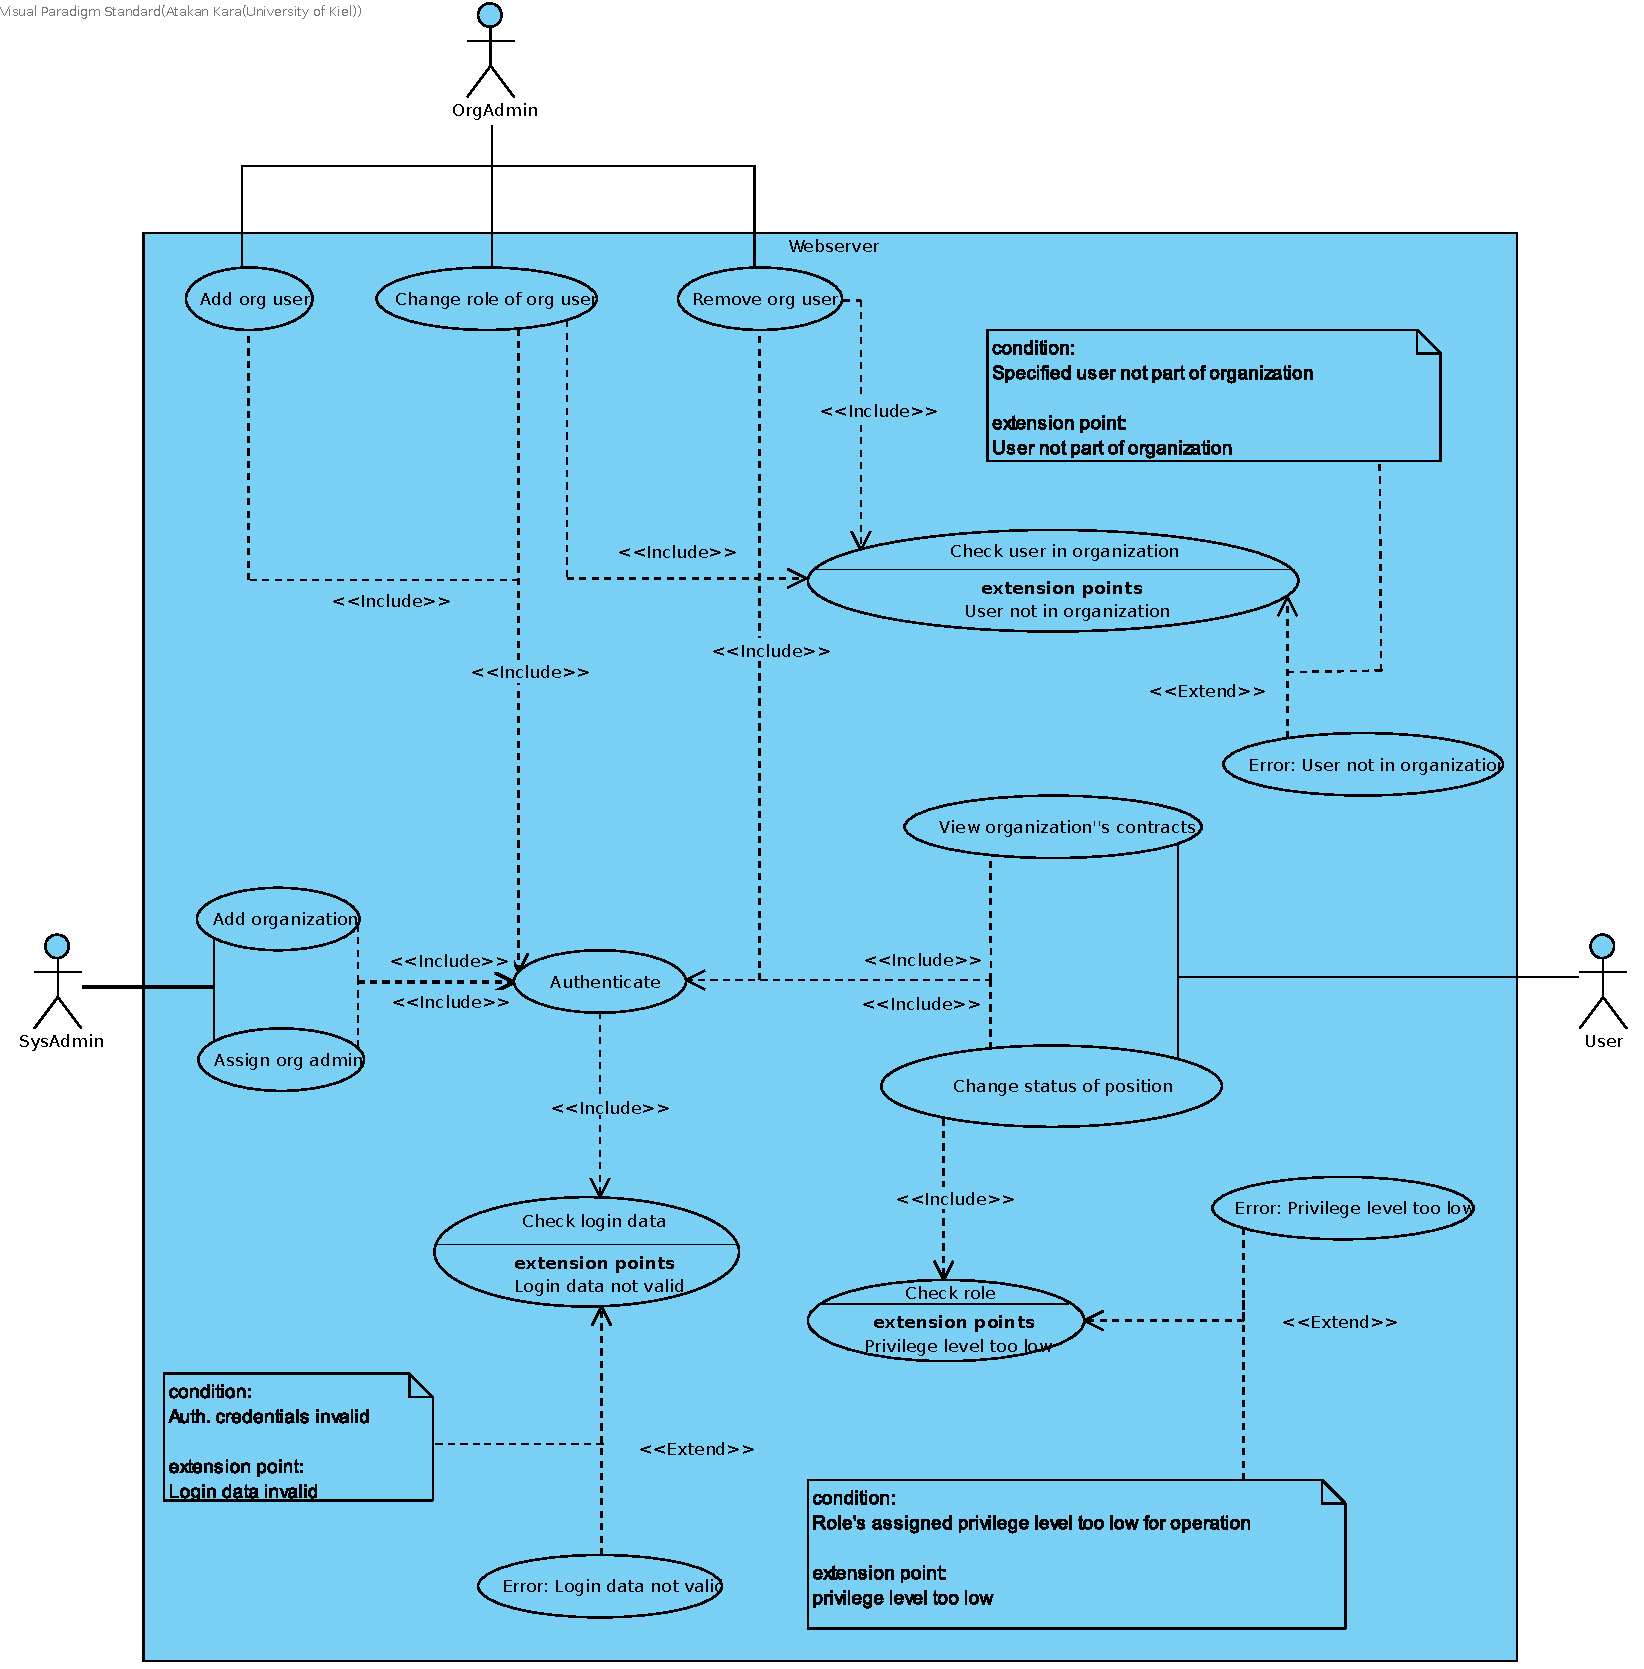
\includegraphics[width=\linewidth]{diagrams/Acc_Management_Web.pdf}
	\caption{Anwendungsfalldiagramm - Account-Management Webserver}
	\label{fig:anwendungsfalldiagramm-acc}
\end{figure}

\newpage

\begin{figure}[h]
	\centering
	\begin{tabularx}{\textwidth}{ X | X }
		\textbf{Anwendungsfall ID} & XX-1 \\ \hline
		\textbf{Anwendungsfallname} & Hier steht ein Name. \\ \hline
		\textbf{Initiierender Akteur} & Informatiker \\ \hline
		\textbf{Weitere Akteure} & Designer, Techniker  \\ \hline
		\textbf{Kurzbeschreibung} & Hier steht eine Kurzbeschreibung.  \\ \hline
		\textbf{Vorbedingungen} & -  \\ \hline
		\textbf{Nachbedingungen} & Y trifft zu.  \\ \hline
		\textbf{Ablauf} &
		\begin{enumerate}
			\item Erster ganzer Satz.
			\item Zweiter ganzer Satz.
		\end{enumerate} \\ \hline
		\textbf{Alternative} &
		\begin{enumerate}
			\item Erster ganzer Satz.
			\item Zweiter ganzer Satz.
		\end{enumerate}  \\ \hline
		\textbf{Ausnahme} &
		\begin{enumerate}
			\item Erster ganzer Satz.
			\item Zweiter ganzer Satz.
		\end{enumerate}  \\ \hline
		\textbf{Benutzte Anwendungsfälle} & YY-1 (oder Name) \\ \hline
		\textbf{Spezielle Anforderungen} & - \\ \hline
		\textbf{Annahmen} & -
	\end{tabularx}
	\caption{Anwendungsfall XX-1}
	\label{fig:anwendungsfall-server-tabelle-xx-1}
\end{figure}

\clearpage

\subsection{Diagrammdarstellung}

\begin{figure}[h]
	\centering
	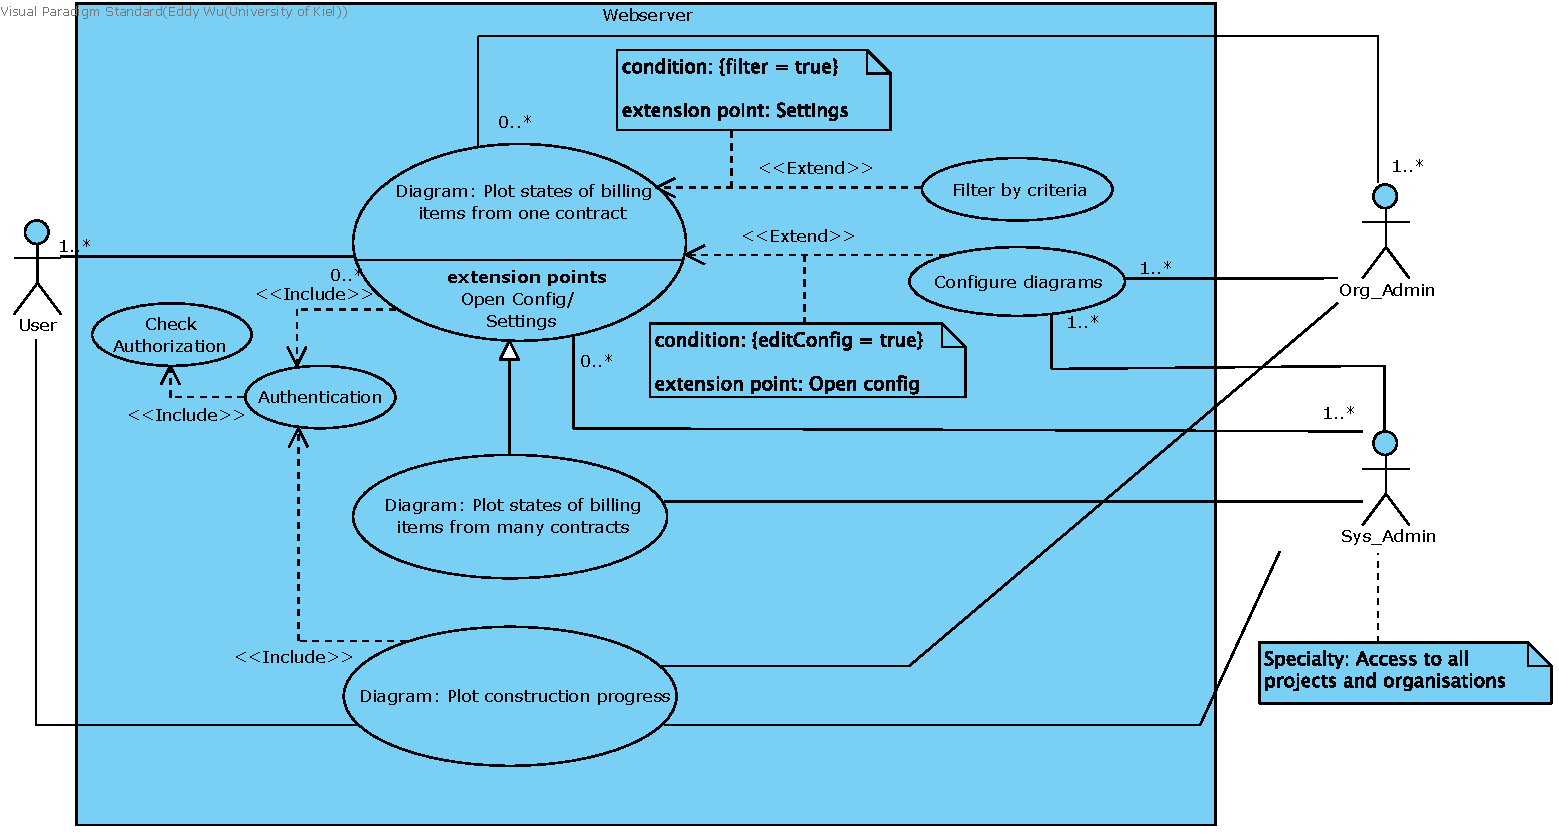
\includegraphics[width=\linewidth]{diagrams/Diagram_Display_Management_Web.pdf}
	\caption{Anwendungsfalldiagramm - Diagrammdarstellung}
	\label{fig:anwendungsfalldiagramm-dia-management}
\end{figure}

\newpage

\begin{figure}[h]
	\centering
	\begin{tabularx}{\textwidth}{ X | X }
		\textbf{Anwendungsfall ID} & XX-1 \\ \hline
		\textbf{Anwendungsfallname} & Hier steht ein Name. \\ \hline
		\textbf{Initiierender Akteur} & Informatiker \\ \hline
		\textbf{Weitere Akteure} & Designer, Techniker  \\ \hline
		\textbf{Kurzbeschreibung} & Hier steht eine Kurzbeschreibung.  \\ \hline
		\textbf{Vorbedingungen} & -  \\ \hline
		\textbf{Nachbedingungen} & Y trifft zu.  \\ \hline
		\textbf{Ablauf} &
		\begin{enumerate}
			\item Erster ganzer Satz.
			\item Zweiter ganzer Satz.
		\end{enumerate} \\ \hline
		\textbf{Alternative} &
		\begin{enumerate}
			\item Erster ganzer Satz.
			\item Zweiter ganzer Satz.
		\end{enumerate}  \\ \hline
		\textbf{Ausnahme} &
		\begin{enumerate}
			\item Erster ganzer Satz.
			\item Zweiter ganzer Satz.
		\end{enumerate}  \\ \hline
		\textbf{Benutzte Anwendungsfälle} & YY-1 (oder Name) \\ \hline
		\textbf{Spezielle Anforderungen} & - \\ \hline
		\textbf{Annahmen} & -
	\end{tabularx}
	\caption{Anwendungsfall XX-1}
	\label{fig:anwendungsfall-server-tabelle-xx-1}
\end{figure}